% Chapter Template

\chapter{Numerical Methods for the Diffusion Equation} % Main chapter title

\label{Chapter3} % Change X to a consecutive number; for referencing this chapter elsewhere, use \ref{ChapterX}
 
%----------------------------------------------------------------------------------------
%	SECTION 1
%----------------------------------------------------------------------------------------

\section{Finite Difference Method for Parabolic PDE's }

%CODE: Heat062017v2.m, fd1d\_heat.m\\
The goal of this document is to look at convergence of finite difference methods for parabolic PDEs of the form 
%%
\begin{subequations} \label{eqn:parabolicPDE}
\begin{eqnarray}
\pd{}{u}{t} - \nabla \cdot(k \nabla u)=f, \;
x \in \Omega, t>0,
\end{eqnarray}
the heat or diffusion equation, where $\Omega$ is open and bounded.  With initial conditions
and boundary conditions:
%%
\begin{eqnarray}
B.C.&\hspace{5mm} u(x,t) =h(t),   &\forall \, x \in \partial\Omega, \, t>0 
\\
I.C.&\hspace{5mm}  u(x,0) = u_0(x) &\forall \, x \in \Omega.
\end{eqnarray}
\end{subequations}
%%
This will be done by looking at two codes. One is a more general code creating during MTH553 at Oregon State University with Professor Adel Faridani Spring 2017. This code allows for implicit, explicit and Crank-Nicolson schemes based on the chosen value of $\mu$. The second code was developed by Professor Peszynska, takes a more in depth look at the implicit method. Some notation differs between methods, but overall methods are very similar.  Both codes use an implicit method that is point centered  difference in space domain and backward difference in time. The error of the implicit and explicit methods is $O(\Delta x^2 + \Delta t)$ and for the Crank-Nicolson  is $O(\Delta x^2 + \Delta t^2)$ .\\
 
%-----------------------------------
%	SUBSECTION 1
%-----------------------------------

\subsection{Multiple Method Code for Equation (\ref{eqn:parabolicPDE}) }
The first code is set up to calculate a numerical solution for 
\begin{subequations}
\begin{eqnarray}
&u_t - k u_{xx} = f(x,t) &x \in (a,b),\, t>0 \\
B.C.&\hspace{5mm} u(a,t) =h_l(t),   \hspace{1cm}   u(b,t) = h_r(t) &t>0
\\
I.C.&\hspace{5mm}  u(x,0) = u_0(x) &x\in(a,b)
\end{eqnarray}
\end{subequations}
where $k$ is a constant. The code is based on the Crank-Nicolson scheme but can be changed to explicit of implicit using the variable $\mu$, where $\mu = 1$ is used for an implicit method, $\mu=0$ for explicit and $\mu = 1/2$ for Crank-Nicolson. The main equation for this scheme is
%
\small
\begin{align} \label{eqn:muparabolicparabolicPDE}
U_j^{n}    - r k\mu\big(U_{j+1}^{n}-2U_j^{n}+U_{j-1}^{n}\big) =&\\
 U_j^{n-1} + rk(1-\mu)&\big(U_{j+1}^{n-1}-2U_j^{n-1}+U_{j-1}^{n-1}\big)
 + \Delta t\big(\mu f_j^{n}+(1-\mu)f_j^{n-1}\big), 
\label{equ matrix Q} \nonumber 
\end{align}
\normalsize
%%
where $r=\frac{\Delta t}{(\Delta x)^2}$. Letting $B$ be the matrix representation of the left hand side of \ref{eqn:muparabolicparabolicPDE} such that $BU^n$ gives the corresponding $j$th component, we get the the following tridiagonal matrix, 
\begin{eqnarray}
B = \begin{bmatrix} 
1+\mu 2 r k & -\mu r k  \\
-\mu r k       & 1+\mu 2 r k& -\mu r k  \\
                    & \ddots           & \ddots & \ddots \\
            & &        -\mu r k  &  1+\mu 2 r k &  -\mu r k  \\
                      &   & &        -\mu r k  &  1+\mu 2 r k   \\
\end{bmatrix},
\end{eqnarray}
we can then write the scheme as 
\begin{eqnarray}
BU^{n} &=& {R}^{n-1}, 
\end{eqnarray}
where both $R$ and $B$ are dependent on $\mu$ and $R$ stands for the right hand side and not to be confused with the residual. Let
\begin{eqnarray}
U^{n} = \begin{bmatrix}
U_1^{n}\\
\vdots\\
U_N^{n}\\
\end{bmatrix}
\hspace{1cm} \text{ and }\hspace{1cm}
{R}^{n-1} = \begin{bmatrix}
R_1^{n-1}\\
\vdots\\
R_N^{n-1}\\
\end{bmatrix}
\end{eqnarray}
where $N$ is the number of time steps subtract 1, i.e. then numbers of points used in the space dimension excluding the boundary points.  
In the code, a matrix $Q$ was used to help calculate $R^{n-1}_j$ in equation  \ref{eqn:matrixQFIparabolicPDE} for $j=1,\dots,N$,
\begin{eqnarray}
Q = \begin{bmatrix} \label{eqn:matrixQFIparabolicPDE}
1-2 r k (1-\mu) & r k (1-\mu)  \\
 r k (1-\mu)        & 1-2 r k (1-\mu) &  r k (1-\mu)   \\
                    & \ddots           & \ddots & \ddots \\
            & &         r k (1-\mu)   &1-2 r k (1-\mu)  &  r k (1-\mu) \\
                      &   & &       r k (1-\mu) &  1-2 r k (1-\mu)    \\
\end{bmatrix}.
\end{eqnarray}

Both $A$ and $Q$ are $N\times N$ matrices.  A vector, $P$, was used to incorporate the boundary conditions 
\begin{eqnarray}
P= 
\begin{bmatrix}
\mu r k g(t_{n}) + r k (1-\mu) h_l(t_{n-1})\\
0\\
\vdots \\
0 \\
\mu r k h(t_{}) n+ r k (1-\mu) h_r(t_{n-1})
\end{bmatrix}.
\end{eqnarray}
The vector $R^{n-1}$ is then calculated using $Q$, $P$, the right hand side equation, $f$, as seen in equation \ref{equn Rm} below. In equation \ref{equn Rm}, $x$ is a vector of the interior  points, length $N$.  Then $R^{n-1}$ and matrix $A$ are used to calculate $U^{n}$ in equation \ref{equn Un}
\begin{eqnarray}
 R^{n-1} &=& QU^{n-1}+P+\Delta t(\mu f(x,t_{n}) +(1-\mu)f(x,t_{n-1}) )\label{equn Rm}\\
    U^{n}& =& B^{-1}R^{n-1} \label{equn Un}.
\end{eqnarray}
The code steps through this process until the specified end time is reached. 
%-----------------------------------
%	SUBSECTION 2
%-----------------------------------
\subsection{Fully Implicit Code for Equation (\ref{eqn:parabolicPDE})}
The main differences between this and the previous method are the way the boundary conditions are implemented and that this method is only implemented fully implicitly. The second code used was provided by Professor Peszynska. The code uses the implicit method to calculate a finite difference approximation of a simple  parabolic two-point boundary value problem $u_t-u_{xx} = f$ as a function with imputes $M, a, b, u_a, u_b, T, dt$ correspondingly number of $x$ steps, left end point, right end point, left boundary condition, right boundary condition, final time and time step size. This code calculates the error and graphs the function as well as showing the first few time step changes. Note that the boundary conditions are treated differently. 


\begin{subequations}
	\begin{eqnarray}
	&u_t-k u_{xx} = f  &x \in (a,b),\, t>0 \label{eqn:DiffusionDir} \\
	B.C.&\hspace{5mm} u(a,t) =h_l(t) = 0,   \hspace{1cm}   u(b,t) = h_r(t)=0 &t>0
	\\
	I.C.&\hspace{5mm}  u(x,0) = u_0(x) &x\in(a,b)
	\end{eqnarray}
\end{subequations}
were $f$ is a function of both $x$ and $t$.

Writing this as a fully implicit numerical method we get
\begin{eqnarray}
U^{n}_j + k \frac{\mytau}{h^2}(2U^{n}_j-U^{n}_{j-1}-U^{n}_{j+1}) =\mytau f+U^{n-1}_j.
\end{eqnarray} 

Writing this out in matrix form we have.

\begin{eqnarray} \label{eqn. impl sch}
 \left( \begin{bmatrix}
	1 &  &  &  &  \\
	& 1 &  &  &  \\
	&  & \ddots &  &  \\
	&  &  & 1 &  \\
	&  &  &  & 1 
	\end{bmatrix}  
	- k \frac{ \mytau}{h^2}  \begin{bmatrix}
	0 &  &  &  &  \\
	1 & -2 & 1 &  &  \\
	& \ddots & \ddots & \ddots &  \\
	&  & 1 & -2 & 1 \\
	&  &  &  &  0
	\end{bmatrix}  \right) \begin{bmatrix}
U^{n}_1 \\
U^{n}_2 \\
\vdots\\
U^{n}_{M}\\
U^{n}_{M+1}

\end{bmatrix}  
= 
 \begin{bmatrix}
0 \\
\mytau f \\
\vdots\\
\mytau f \\
0
\end{bmatrix}  
+
 \begin{bmatrix}
0 \\
U^{n-1}_2 \\
\vdots\\
U^{n-1}_{M} \\
0 
\end{bmatrix} 
\end{eqnarray}

and let 
\begin{center}
$ B = \begin{bmatrix}
1 &  &  & & \\
-k \frac{\mytau}{h^2} & 1+2 k \frac{\mytau}{h^2} & -k \frac{\mytau}{h^2} & & \\
& \ddots & \ddots & \ddots \\
& &-k \frac{\mytau}{h^2} & 1+2 k \frac{\mytau}{h^2} & -k \frac{\mytau}{h^2}   \\
& &  &  & 1 
\end{bmatrix}  $
\end{center}
then if $C$ is a vector of length $M$ with $c$ in all entries except the first and last entries which are zero. Then equation (\ref{eqn. impl sch}) can be rewritten as
\begin{eqnarray}
 B U^{n} = \mytau f(\mathbf{x},t_n) +U^{n-1}.
\end{eqnarray}
Where $\mathbf{x}$ is the containing all $x$ nodes. 

For $g(u)=1$, i.e. $c=-1$, the numerical solution for two values of $\varepsilon$ and the initial value is shown in Figure \ref{fig:FIdirBCex1}. For this example $a=0$, $b=1$, $t_{final}=1$ and $\mytau = h^2$.  Figure \ref{fig:FIdirBCex1} was created in Matlab using the build in $\setminus$ function,
\begin{eqnarray} \label{eqn. ACSolveForUn}
 U^{n} = B \setminus \left( \mytau f(\mathbf{x},t_n)  +U^{n-1} \right)
\end{eqnarray}
for each time step.  %%% code:  Cahn_Allenv4_3 and Cahn_Allenv4_Comparison1

		\begin{figure}[H]
		\centering
		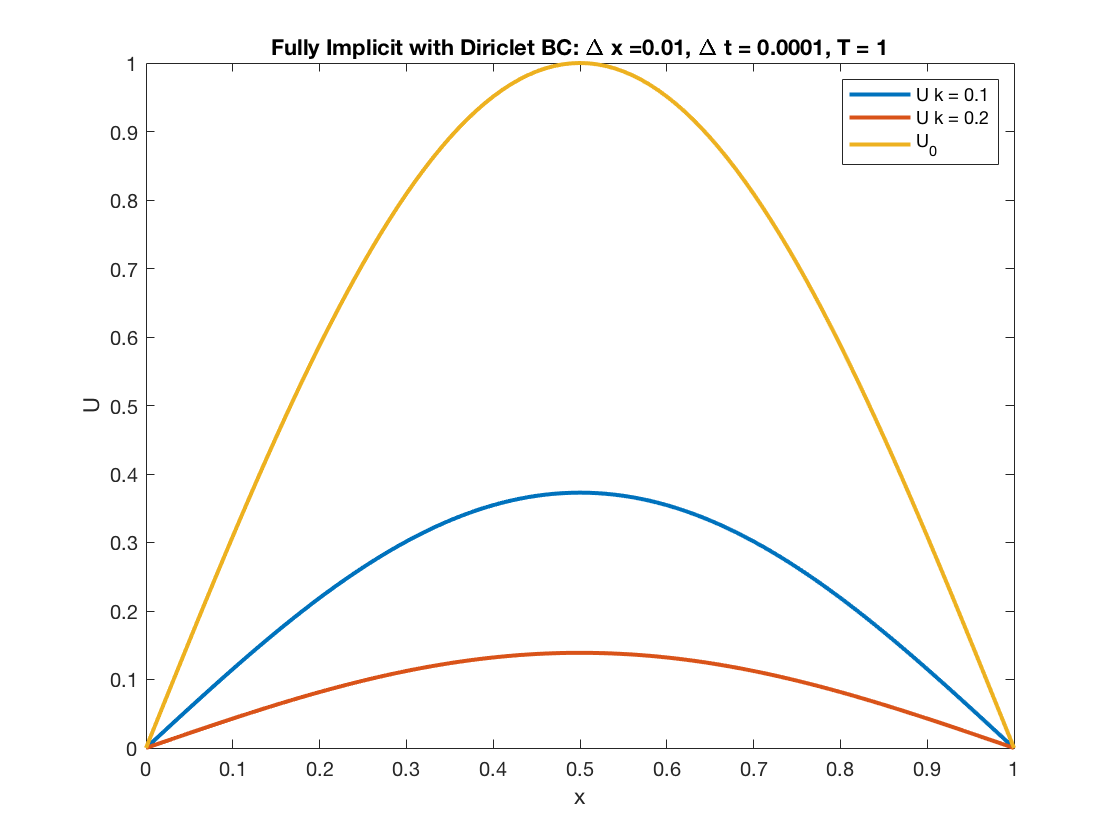
\includegraphics[width=.6\textwidth]{FIdirBCex1.png}
		\caption{Numerical solution using fully implicit finite difference code for the linear diffusion equation where $f=0$, $a=0$, $b=1$, $T=t_{final}=1$, $u_0 = \sin(\pi x) $. Plotted are numerical solutions for two diffusion coefficients, $k=0.1$ and $k=0.2$.}
		\label{fig:FIdirBCex1}
		\end{figure}


%-----------------------------------
%	SUBSECTION 3
%-----------------------------------
\subsection{Convergence Results}
% CODE: Heat062017v2.m, fd1d\_heat.m\\
The first example used was the basic example $u_t-u_{xx}=0$, $u(x,0)=u_{int}(x)= \sin(\pi x) e^{- \pi^2 t}$ on $(0,1)$ and $u|_{\partial u} = u_D=0$. Note that the notation differs between methods.  and the max difference for each graph is listed below the graph.

	Table \ref{tab:conv1} below shows the error and calculated order of accuracy for $h$, $\alpha$ for given $h$ and $\tau$ using the first code with $\mu = 1$ for an implicit method. These values were compared to the second code The error value $e_{\infty}$ was calculated using the known solution, $\hat{U}=U_{exact}$.  In words, $e_{\infty} $ was calculated by taking the maximum absolute difference at each time step then taking the maximum of all the time steps. In symbols, $e_{\infty} = \max_n \max_j  |\hat{U}_j^n-U_j^n|.$ The order of accuracy was calculated using 
	$$\alpha_2 = \frac{\log e_1-\log e_2}{\log h_1 - \log h_2}$$
	where the lower index refers to the row of the value.  \\
	\indent \textbf{Q:} Why are we using $h$ and not $\tau$ to calculate $\alpha$? 
    \\
    For optimal convergence you set $\tau$ to depend on $h$ in some predefined way, so there is only one parameter.\\
	\indent \textbf{Q:} Is there an optimal way to space $h$ efficiently calculate $\alpha$? 
    \\
    The easiest way for ``eyeball'' convergence order checking is to space $h$ with a factor of 10. But any other way will work.
    \\
	In the table $\tau \sim h^2$. The first two values were the same for both methods, the third error value in the table was calculated using just the second code since the first took too long to compile. 
 
 %%%%%%
    \begin{table}[H]
	\begin{center}
		\begin{tabular}{ | c | c | c | c |}
			\hline
			$h$ & $\tau$ & $e_{\infty} $ & $\alpha$ \\ 
			\hline
			 0.1 & 0.01 & 0.0203 & - \\  
			\hline
			 0.01 & 0.0001 &  2.1171e-04 & 1.9822   \\
			 \hline
			 0.001 & 1.00e-06 &  2.1180e-06 &  1.9998  \\
			\hline
		\end{tabular}
        \caption{Error results of max norm.}
        \label{tab:conv1}
	\end{center}
\end{table}
%%

Table \ref{tab:conv2} shows the error results of the $\ell_2$ norm in both time and space numbers. These numbers were calculated using the built in norm function in MATLAB. 
 \begin{table}[H]
	\begin{center}

		\begin{tabular}{ | c | c | c | c |}
			\hline
			$h$ & $\tau$ & $e_{2} $ & $\alpha$ \\ 
			\hline
			0.1 & 0.01 & 0.06308 & - \\  
			\hline
			0.01 & 0.0001 &  0.006477 &  0.9889  \\
			\hline
			0.001 & 1.00e-06 &  0.0205 &   0.4999 \\
			\hline
		\end{tabular}
        \caption{Error results of $\ell_2$ norm}    
        \label{tab:conv2} 
	\end{center}
   \end{table}
   
%----------------------------------------------------------------------------------------
%	SECTION 2
%----------------------------------------------------------------------------------------
   
   \section{Nonlinear Diffusion Equation, Fully Implicit}
   %
%-----------------------------------
%	SUBSECTION 1
%-----------------------------------
\subsection{Nonlinear Diffusion Equation with Dirichlet Boundary Conditions}
   In preparation to work with the phase field model, this section will discuss nonlinear diffusion equations of the form 
%
\begin{subequations}
	\begin{eqnarray}
	&u_t-\varepsilon u_{xx}+\frac{1}{\varepsilon}g(u) = f  &x \in (a,b),\, t>0 \label{eqn. ACexmple} \\
	B.C.&\hspace{5mm} u(a,t) =h_l(t) = 0,   \hspace{1cm}   u(b,t) = h_r(t)=0 &t>0
	\\
	I.C.&\hspace{5mm}  u(x,0) = u_0(x) &x\in(a,b)
	\end{eqnarray}
\end{subequations}
were $f$ is a function of both $x$ and $t$ and $\varepsilon$ is a scalar constant. The first example that will be discussed will have $f = 0$. The discretization used for this problem was a fully implicit method,
\begin{eqnarray}
U^{n}_j-U^{n-1}_j + \varepsilon\frac{ \mytau}{h^2}(2U^{n}_j-U^{n}_{j-1}-U^{n}_{j+1})+\frac{\mytau}{\varepsilon}g(U^n_j) =0 \label{eqn. DirImpHomCA},
\end{eqnarray} 
where $h = \frac{b-a}{M}$ is the uniform step size in space and thus $j=1,\dots,M+1$. Then in the time domain, $\mytau$ is the uniform step size. 


Next, we consider when $g(u)$ is not constant and $f \ne 0$. For example, 
\begin{subequations}
	\begin{eqnarray}
	&u_t-\varepsilon u_{xx}+\frac{1}{\varepsilon}g(u) = f  &x \in (0,1),\, t>0  \\
	B.C.&\hspace{5mm} u(0,t) = 0,   \hspace{2cm}   u(1,t) =0 &t>0
	\\
	I.C.&\hspace{5mm}  u(x,0) = u_0(x)=sin(\pi x) &x\in(0,1)
	\end{eqnarray}
\end{subequations}
%
where 
\begin{subequations}
\begin{align}
 g(u) =& u^3-u \\
 f(x,t) =& \sin(\pi x)+\varepsilon \pi^2 (t+1) \sin(\pi x) \\ & \hspace{3cm}+\frac{1}{\varepsilon} \Big((t+1)\sin(\pi x)-\big((t+1)\sin(\pi x)\big)^3\Big).
\end{align}
\end{subequations}
%
The exact solution for this system of equations is 
\begin{eqnarray}
u = (t+1)\sin(\pi x).
\end{eqnarray} 
Because $g(u)$ is not linear in $u$, using a fully implicit scheme requires an iterative method. Consider the method in (\ref{eqn. CahnAllenNewton})
\begin{eqnarray} \label{eqn. CahnAllenNewton}
U^{n}_j-U^{n-1}_j + \varepsilon \frac{ \mytau}{h^2}(2U^{n_k}_j-U^{n_k}_{j-1}-U^{n_k}_{j+1})+\frac{\mytau}{\varepsilon}g(U^{n_k}_j) = \mytau f,
\end{eqnarray} 
where $f = f(x_j,t_n)$ and $n_k$ represents the time step and the Newton iteration, i.e. $n$ is the time step and the subscript $k$ is the Newton iteration. For detail on Newton's Method see section \ref{Sect:Newton'sMethod}. The initial guess used at each time step was the previous time step, $n-1$, so $U^{n_0} = U^{n-1}$. The 2-grid-norm was used to calculate the norm of the residual. In this case the accuracy was set to $10e{-12}$, thus the norm of the residual needed to be less $10e{-12}$ in order for the current iteration to be accepted as the numerical solution. The tolerance and the max iterations were set leniently at 100 and 25 respectively.  

The residual, in this case, for the interior spacial notes is
\begin{eqnarray}
R_j^{n_k} = U^{n}_j-U^{n-1}_j + \varepsilon \frac{ \mytau}{h^2}(2U^{n_k}_j-U^{n_k}_{j-1}-U^{n_k}_{j+1})+\frac{\mytau}{\varepsilon}g(U^{n_k}_j) - \mytau f(x_j,t_n)
\end{eqnarray}
and for the boundary

\begin{align}
R_{1}^{n_k} =& U_1^{n_{k}}-u(x_1,t_n) \\
R_{M+1}^{n_k} =& U_{M+1}^{n_k} - u(x_{M+1},t_n) 
\end{align}
In this case $u(x_1,t_n) =  u(x_{M+1},t_n) =0$ for all $t_n >0$. The Jacobian is as follows
\begin{center}
$ J = \begin{bmatrix}
1 &  &  & & \\
-\varepsilon \frac{\mytau}{h^2} & 1+2 \varepsilon \frac{\mytau}{h^2} +\frac{1}{\varepsilon}g'(U_2^{n_k})& -\varepsilon \frac{\mytau}{h^2} & & \\
& \ddots & \ddots & \ddots \\
& &-\varepsilon \frac{\mytau}{h^2} & 1+2 \varepsilon \frac{\mytau}{h^2} +\frac{1}{\varepsilon}g'(U_M^{n_k})& -\varepsilon \frac{\mytau}{h^2}   \\
& &  &  & 1 
\end{bmatrix}.  $
\end{center}


%
%-----------------------------------
%	SUBSECTION 2
%-----------------------------------
\subsection{Nonlinear Diffusion Equation with Neumann Boundary Conditions}

%Code: Cahn_Allenv7_2
The boundary condition is the only thing that differs between Allen-Cahn heat equation fully implicit with Neumann boundary condition method and the fully implicit method with Dirichlet boundary conditions. The initial boundary value problem now becomes
\begin{subequations}
	\begin{eqnarray}
	&u_t-\varepsilon u_{xx}+\frac{1}{\varepsilon}g(u) = f  &x \in (a,b),\, t>0  \\
	B.C.&\hspace{5mm} u'(a,t) = 0,   \hspace{5mm}   u'(b,t) =0 &t>0
	\\
	I.C.&\hspace{5mm}  u(x,0) = u_0(x) &x\in(a,b)
	\end{eqnarray}
\end{subequations}

There are only a couple of changes between the code for Neumann and Dirichlet boundary condition. The change are, the boundary conditions and the Jacobian. In the code, this is what differs for the boundary conditions. First is the center followed by the boundary conditions
\begin{eqnarray}
R_j^{n_k} = U^{n}_j-U^{n-1}_j + \varepsilon \frac{ \mytau}{h^2}(2U^{n_k}_j-U^{n_k}_{j-1}-U^{n_k}_{j+1})+\frac{\mytau}{\varepsilon}g(U^{n_k}_j) - \mytau f(x_j,t_n)
\end{eqnarray}
and for the boundary
\begin{align}
R_{1}^{n_k} =& U_1^{n_{k}}+\varepsilon \frac{\mytau}{h^2} (2 U_1^{n_k}-2 U_2^{n_k}) +\frac{\mytau}{\varepsilon} g(U_1^{n_k})-\mytau f(x_1,t_n)-U_1^{n-1}\\ 
R_{M+1}^{n_k} =& U_{M+1}^{n_k}+\varepsilon \frac{\mytau}{h^2} (2 U_{M+1}^{n_k}-2 U_{M}^{n_k})+\frac{\mytau}{\varepsilon} g(U_{M+1}^{n_k})-\mytau f(x_{M+1},t_n)-U_{M+1}^{n-1}
\end{align}
The Jacobain for this method is
\scriptsize{
\begin{center}
$ J = \begin{bmatrix}
1+2\varepsilon \frac{\mytau}{h^2}+\frac{\mytau}{\varepsilon} g'(U_1^{n_k})  & -2\varepsilon \frac{\mytau}{h^2} &  & & \\
-\varepsilon \frac{\mytau}{h^2} & 1+2 \varepsilon \frac{\mytau}{h^2} +\frac{1}{\varepsilon}g'(U_2^{n_k})& -\varepsilon \frac{\mytau}{h^2} & & \\
& \ddots & \ddots & \ddots \\
& &-\varepsilon \frac{\mytau}{h^2} & 1+2 \varepsilon \frac{\mytau}{h^2} +\frac{1}{\varepsilon}g'(U_M^{n_k})& -\varepsilon \frac{\mytau}{h^2}   \\
& &  &  -2\varepsilon \frac{\mytau}{h^2} & 1+2\varepsilon \frac{\mytau}{h^2}+\frac{\mytau}{\varepsilon} g'(U_{M+1}^{n_k}) 
\end{bmatrix}.  $
\end{center} }
\normalsize


%----------------------------------------------------------------------------------------
%	SECTION 3
%----------------------------------------------------------------------------------------
\section{Nonlinear Diffusion Equation, Time Lagging}
%
For the time lagging method, the function $g(u)$ is evaluated at $U^{n-1}$, thus equation (\ref{eqn. CahnAllenNewton}) becomes
\begin{eqnarray} \label{eqn. CahnAllenTimeLagging}
U^{n}_j-U^{n-1}_j + \varepsilon \frac{ \mytau}{h^2}(2U^n_j-U^n_{j-1}-U^n_{j+1})+\frac{\mytau}{\varepsilon}g(U_j^{n-1} ) =\mytau f.
\end{eqnarray} 
This method does not require an iterative method and can be solved similarly to how it is in equation (\ref{eqn. ACSolveForUn}), however this method can deviate from the true solution more than the fully implicit method. 


%----------------------------------------------------------------------------------------
%	SECTION 5
%----------------------------------------------------------------------------------------
\section{Allen-Cahn Heat Equation Splitting Method with Neumann Boundary Conditions} \label{Sect. Allen-Cahn Heat Equation Splitting Method with Neumann Boundary Conditions} 
The main idea for the splitting method is to break up the nonlinearity, in our case the $g(u) =u^3-u$, into an expansive and an contractive term and 
evaluate the contractive term implicitly and the expansive term explicitly. This is more explicitly discussed in the section \ref{Sect:Splitting}. The first splitting method used is 
\begin{eqnarray} \label{eqn. CahnAllenSplitting1}
U^{n}_j-U^{n-1}_j + \varepsilon \frac{ \mytau}{h^2}(2U^n_j-U^n_{j-1}-U^n_{j+1})+\frac{\mytau}{\varepsilon}5 U_j^{n}  =\frac{\mytau}{\varepsilon}6 U_j^{n-1}- \frac{\mytau}{\varepsilon}(U_j^{n-1})^3+\mytau f.
\end{eqnarray} 



%----------------------------------------------------------------------------------------
%	SECTION 5
%----------------------------------------------------------------------------------------
\section{Comparing Fully Implicit, Time Lagging, and the Splitting Methods for the Cahn-Allen Heat Equation} \label{Sect. Comparing Fully Implicit, Time Lagging, and the Splitting Methods for the Cahn-Allen Heat Equation} 
This section compared the fully implicit, time lagging, and the splitting methods for the Cahn-Allen heat equation. All methods used Neumann boundary conditions, thus the initial boundary value problem for this section is 
\begin{subequations}
	\begin{eqnarray}
	&u_t-\varepsilon u_{xx}+\frac{1}{\varepsilon}g(u) = f  &x \in (a,b),\, t>0  \\
	B.C.&\hspace{5mm} u'(a,t) = 0,   \hspace{5mm}   u'(b,t) =0 &t>0
	\\
	I.C.&\hspace{5mm}  u(x,0) = u_0(x) &x\in(a,b)
	\end{eqnarray}
\end{subequations}
where unless otherwise specified $a=0$ and $b=1$. This section will looks at a few specific examples with different initial conditions. The first exam will have the initial condition of $u_0\left( (a, \frac{b-a}{2}) \right)= -1$ for the first half of the interval $(0,1)$ and the second half will be one, $u_0\left( [\frac{b-a}{2},b) \right)= 1$. If there are an odd number of nodes, then the middle node is included in the second half and given the initial value one. 
		\begin{figure}[H]
		\centering
		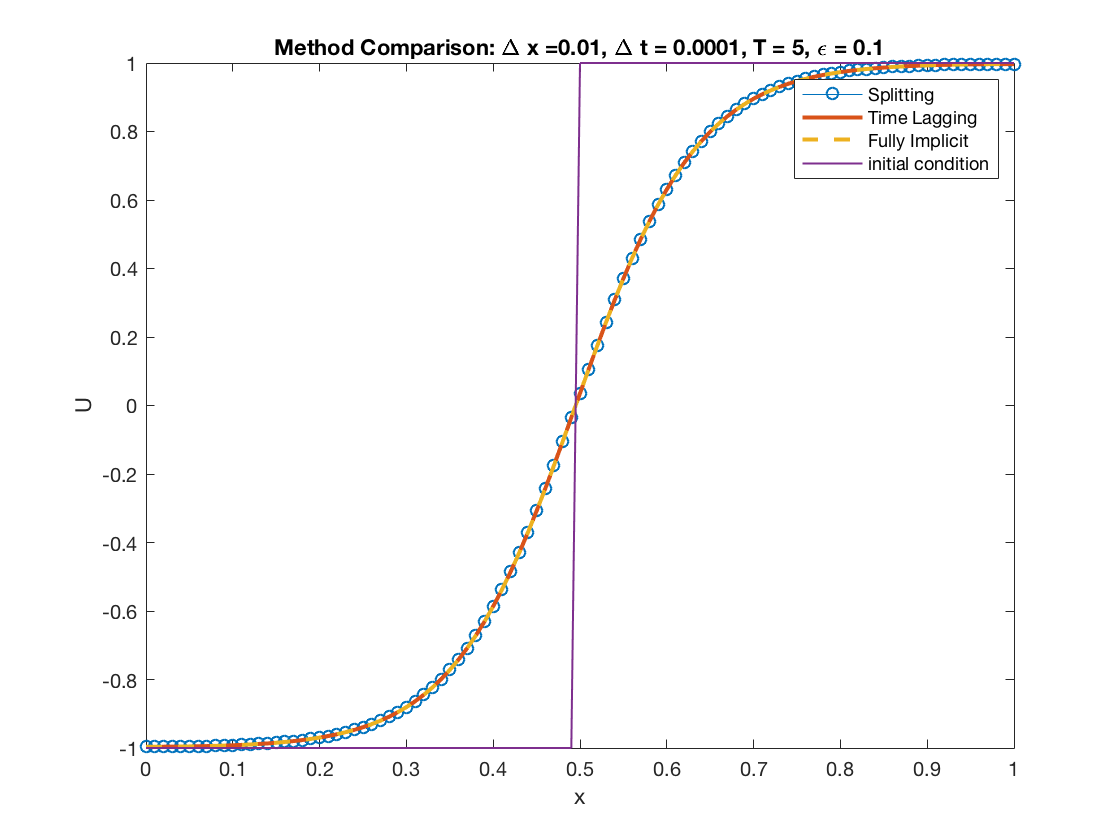
\includegraphics[width=.45\textwidth]{MethComUo1e01.png}
        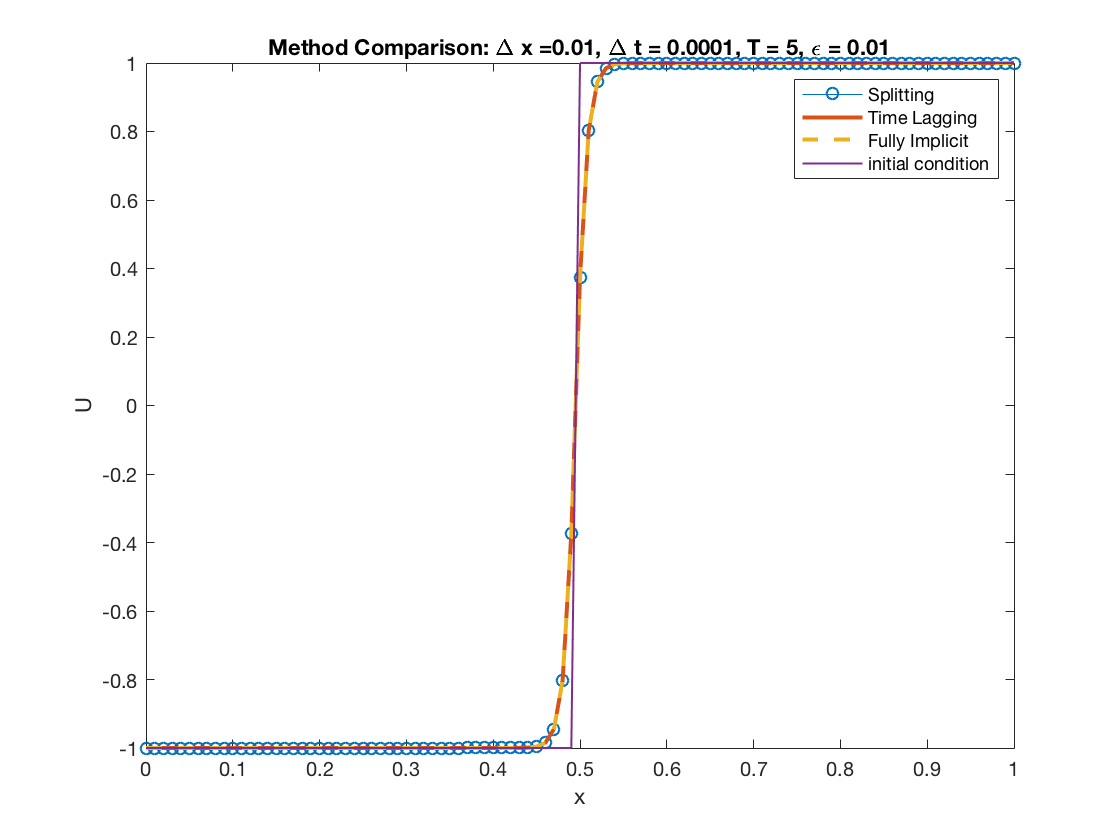
\includegraphics[width=.45\textwidth]{MethComUo1e001.png}
		\caption{Plots for all three methods and two different values of $\varepsilon$ but keeping all other inputs the same. }
		\label{fig:MethComUo1}
		\end{figure}

The initial value for this example was $u_0=\frac{1}{3}\cos(7\pi x )+\frac{1}{3}\cos(29\pi x )+\frac{1}{3} \cos(\pi x)$   
		\begin{figure}[H]
		\centering
		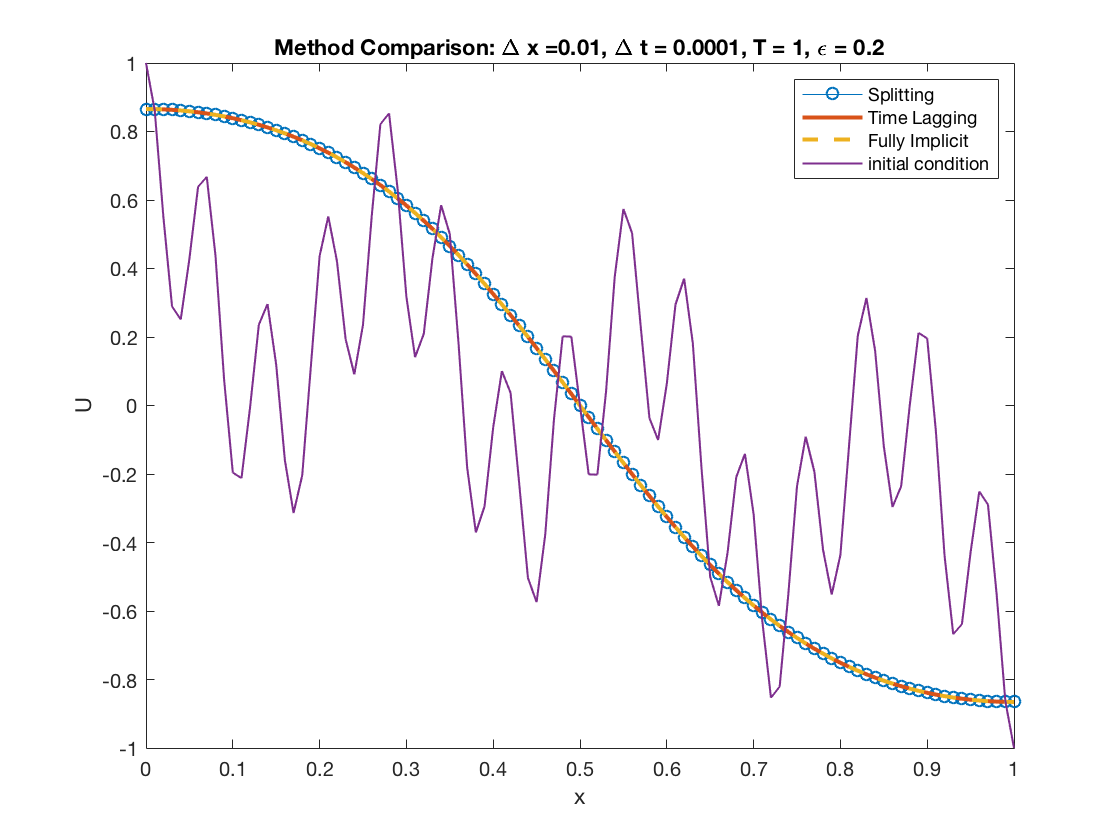
\includegraphics[width=.6\textwidth]{MethComUo2e02.png}
        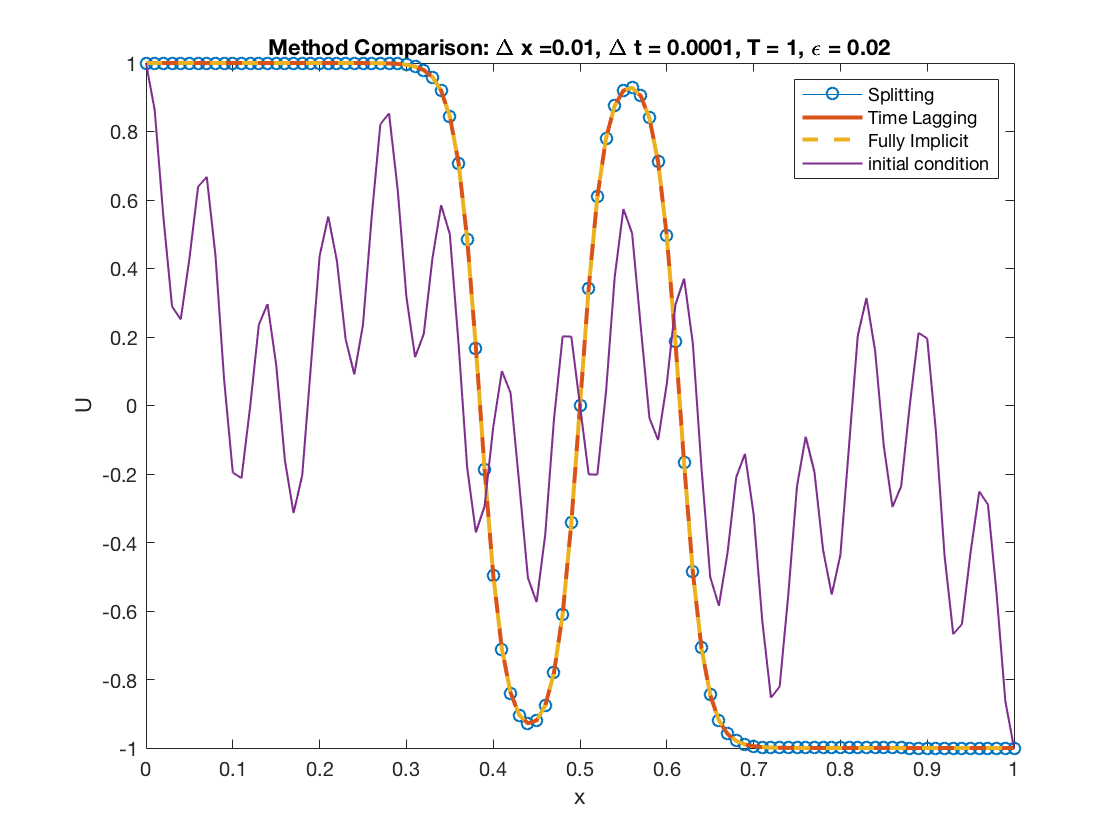
\includegraphics[width=.6\textwidth]{MethComUo2e002.png}
		\caption{Plots for all three methods and two different values of $\varepsilon$ but keeping all other inputs the same. }
		\label{fig:MethComUo2}
		\end{figure}
For the case that $\varepsilon = 0.2$, the $||U_{FI}-U_{S}||_{2, \Delta} = 9.2e{-5}$ while $||U_{FI}-U_{TL}||_{2, \Delta} = 8.0e{-7}$ where $||\cdot||_{2, \Delta}$ is the grid 2-norm and in this case is taken at the final time, $t=T=1$, and $U_{FI}$ is $U_{final}$ using the fully implicit method. 






        